
% %%%%%%%%%%%%%%%%%%%%%%%%%%%%%%%%%%%%%%%%%%%%%%%%%%%%%%%%%%%%%%%%%%%%%
% \savegeometry{beamergeo}
% \begin{emptyframe}
%     \frametitle{Truncated mass divergence in the Mott metal NiS$_2$}
%     \centerline{ \includegraphics[width=0.95\columnwidth]{\data/NiS2/FiguresNiS2/NiS2Summary.pdf}}
% \vspace{-1 em}
% \vfill
% \centerline{\makebox[\linewidth]{\rule{0.85\textwidth}{0.4pt}}}
% \centerline{\scriptsize Semeniuk {\it et al.} PNAS e2301456120 (2023)}
% \end{emptyframe}
% \loadgeometry{beamergeo}

% %%%%%%%%%%%%%%%%%%%%%%%%%%%%%%%%%%%%%%%%%%%%%%%%%%%%%%%%%%%%%%%%%%%%%
% \savegeometry{beamergeo}
% \begin{emptyframe}
%     \frametitle{Superconductivity in the Hund's metals (Y/Lu)Fe$_2$Ge$_2$}
%     \centerline{ \includegraphics[width=0.85\columnwidth]{\data/YFe2Ge2/FiguresYFG/Overview/YFe2Ge2Summary.pdf}}
% \vspace{-1 em}
% \vfill 
% \centerline{\makebox[\linewidth]{\rule{0.85\textwidth}{0.4pt}}}
% \centerline{\scriptsize Chen {\it et al.} PRL {\bf 125,} 237002 (2020), Baglo {\it et al.} PRL {\bf 129,} 046402 (2022)}
% \end{emptyframe}
% \loadgeometry{beamergeo}

% %%%%%%%%%%%%%%%%%%%%%%%%%%%%%%%%%%%%%%%%%%%%%%%%%%%%%%%%%%%%%%%%%%%%%
% \savegeometry{beamergeo}
% \begin{emptyframe}
%     \frametitle{Quantum oscillations in the new superconductor UTe$_2$}
%     \centerline{ \includegraphics[width=0.75\columnwidth]{\data/UTe2/FiguresUTe2/Overview/SummaryUTe2-2.png}}
% \vspace{-1 em}
% \vfill 
% \centerline{\makebox[\linewidth]{\rule{0.85\textwidth}{0.4pt}}}
% \centerline{\scriptsize Eaton Nature Comm., arXiv:2302.04758 (2023), Wu arXiv:2305.19033 (2023), Weinberger arXiv:2307.00568 (2023)}
% \end{emptyframe}
% \loadgeometry{beamergeo}



%%%%%%%%%%%%%%%%%%%%%%%%%%%%%%%%%%%%%%%%%%%%%%%%%%%%%%%%%%%%%%%%%%%%%
\savegeometry{beamergeo}
\begin{emptyframe}
%\begin{frame}[plain,label=TitlePage]
\begin{center}
\textcolor{Blue}{Electronic and structural instabilities} \\
\vspace{0.5em}
{\footnotesize F. M. Grosche} \\
{\footnotesize \em Cavendish Laboratory, Cambridge} \\
\vspace{0.1em}
\end{center}
\vspace{0.0em}
%\centerline{\multiinclude[<visible@+-| +->][format=pdf,graphics={width=\columnwidth}]{\Figures/FermInstab/QPTScenariosHostGuest2}}
% \setbeamercovered{invisible}
% \begin{tikzpicture}
    %     \node[anchor=south west,inner sep=0] (image) at (0,0) {
        \centerline{ 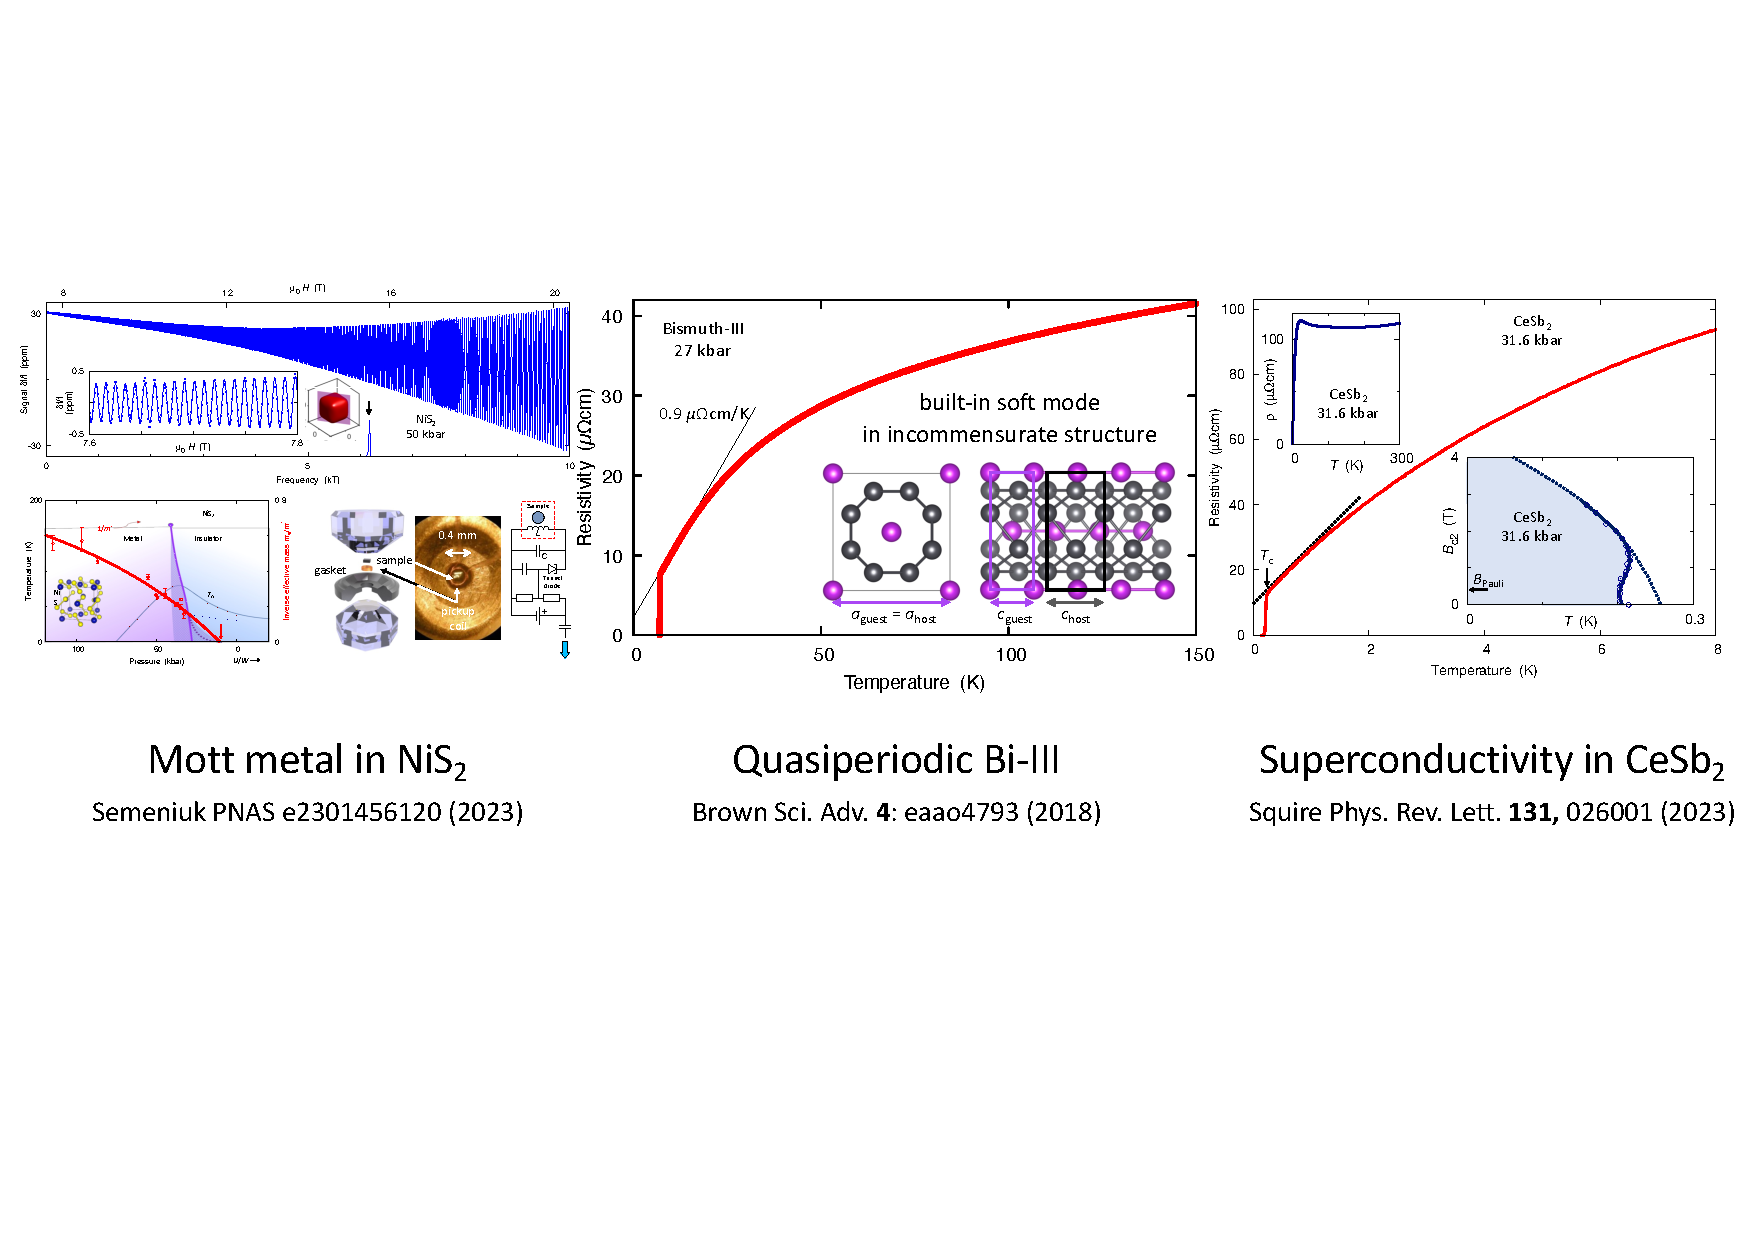
\includegraphics[width=\columnwidth]{IntroPicture2}}
    %     };
    %     \pause
    %     \begin{scope}[x={(image.south east)},y={(image.north west)}]
        %         \draw[Blue,line width=1 mm] (0, 1)--(1, 0);
        %         \draw[Blue,line width=1 mm] (0, 0)--(1, 1);
    %     \end{scope}
% \end{tikzpicture}

\vspace{1em}
\begin{itemize}
    %   \item<1-> Recent projects in Cambridge Quantum Matter group
    \item<1-> High pressure quantum oscillation measurements in NiS$_2$
    \item<2-> Anomalous low-$T$ resistivity in quasiperiodic Bi-III
    \item<3-> CeSb$_2$, a new high pressure superconductor
\end{itemize}
\setbeamercovered{transparent}
\end{emptyframe}
\loadgeometry{beamergeo}



%%% Local Variables: 
%%% mode: latex
%%% TeX-master: "GroTalk.ho"
%%% End: 
